\documentclass{exam}
\usepackage{xcolor, minted, graphicx, fontspec}
\setmainfont{Open Sans}
\graphicspath{ {./images} }

\author{Jordy Alkema}
\title {Homework Week 1}

\begin{document}
\maketitle

\section{Review}
\begin{questions}
	\question
	\begin{parts}
		\part
		Databases die geoptimaliseerd zijn om data op te slaan waaraan een tijd zit gekoppeld. In tegenstelling tot een normale database hangt aan elke waarde een timestamp. Dit is nuttig als er grote hoeveelheden data moeten worden opgeslagen die tijdsgevoelig zijn. Zoals bijvoorbeeld de temperaturen van een sensor elke 5 seconden.
		\part
		\begin{minted}[bgcolor=lightgray]{sql}
            % _ [] ^ -
        \end{minted}
		\part
		\begin{parts}
			\part
			3
			\part
			a is niet deel van de GROUP BY clause maar wordt ook niet gebruikt door een aggregate function zoals SUM
		\end{parts}
		\part
		Een outer join geeft alle waardes terug, ook degene die niet een equivalent hebben in alle tabellen. Het is niet altijd mogelijk deze te vervangen door een inner join aangezien waardes die niet overeenkomen tussen beide tabellen hierdoor worden weggelaten.
	\end{parts}
\end{questions}
\section{Questions}
\begin{questions}
	\question
	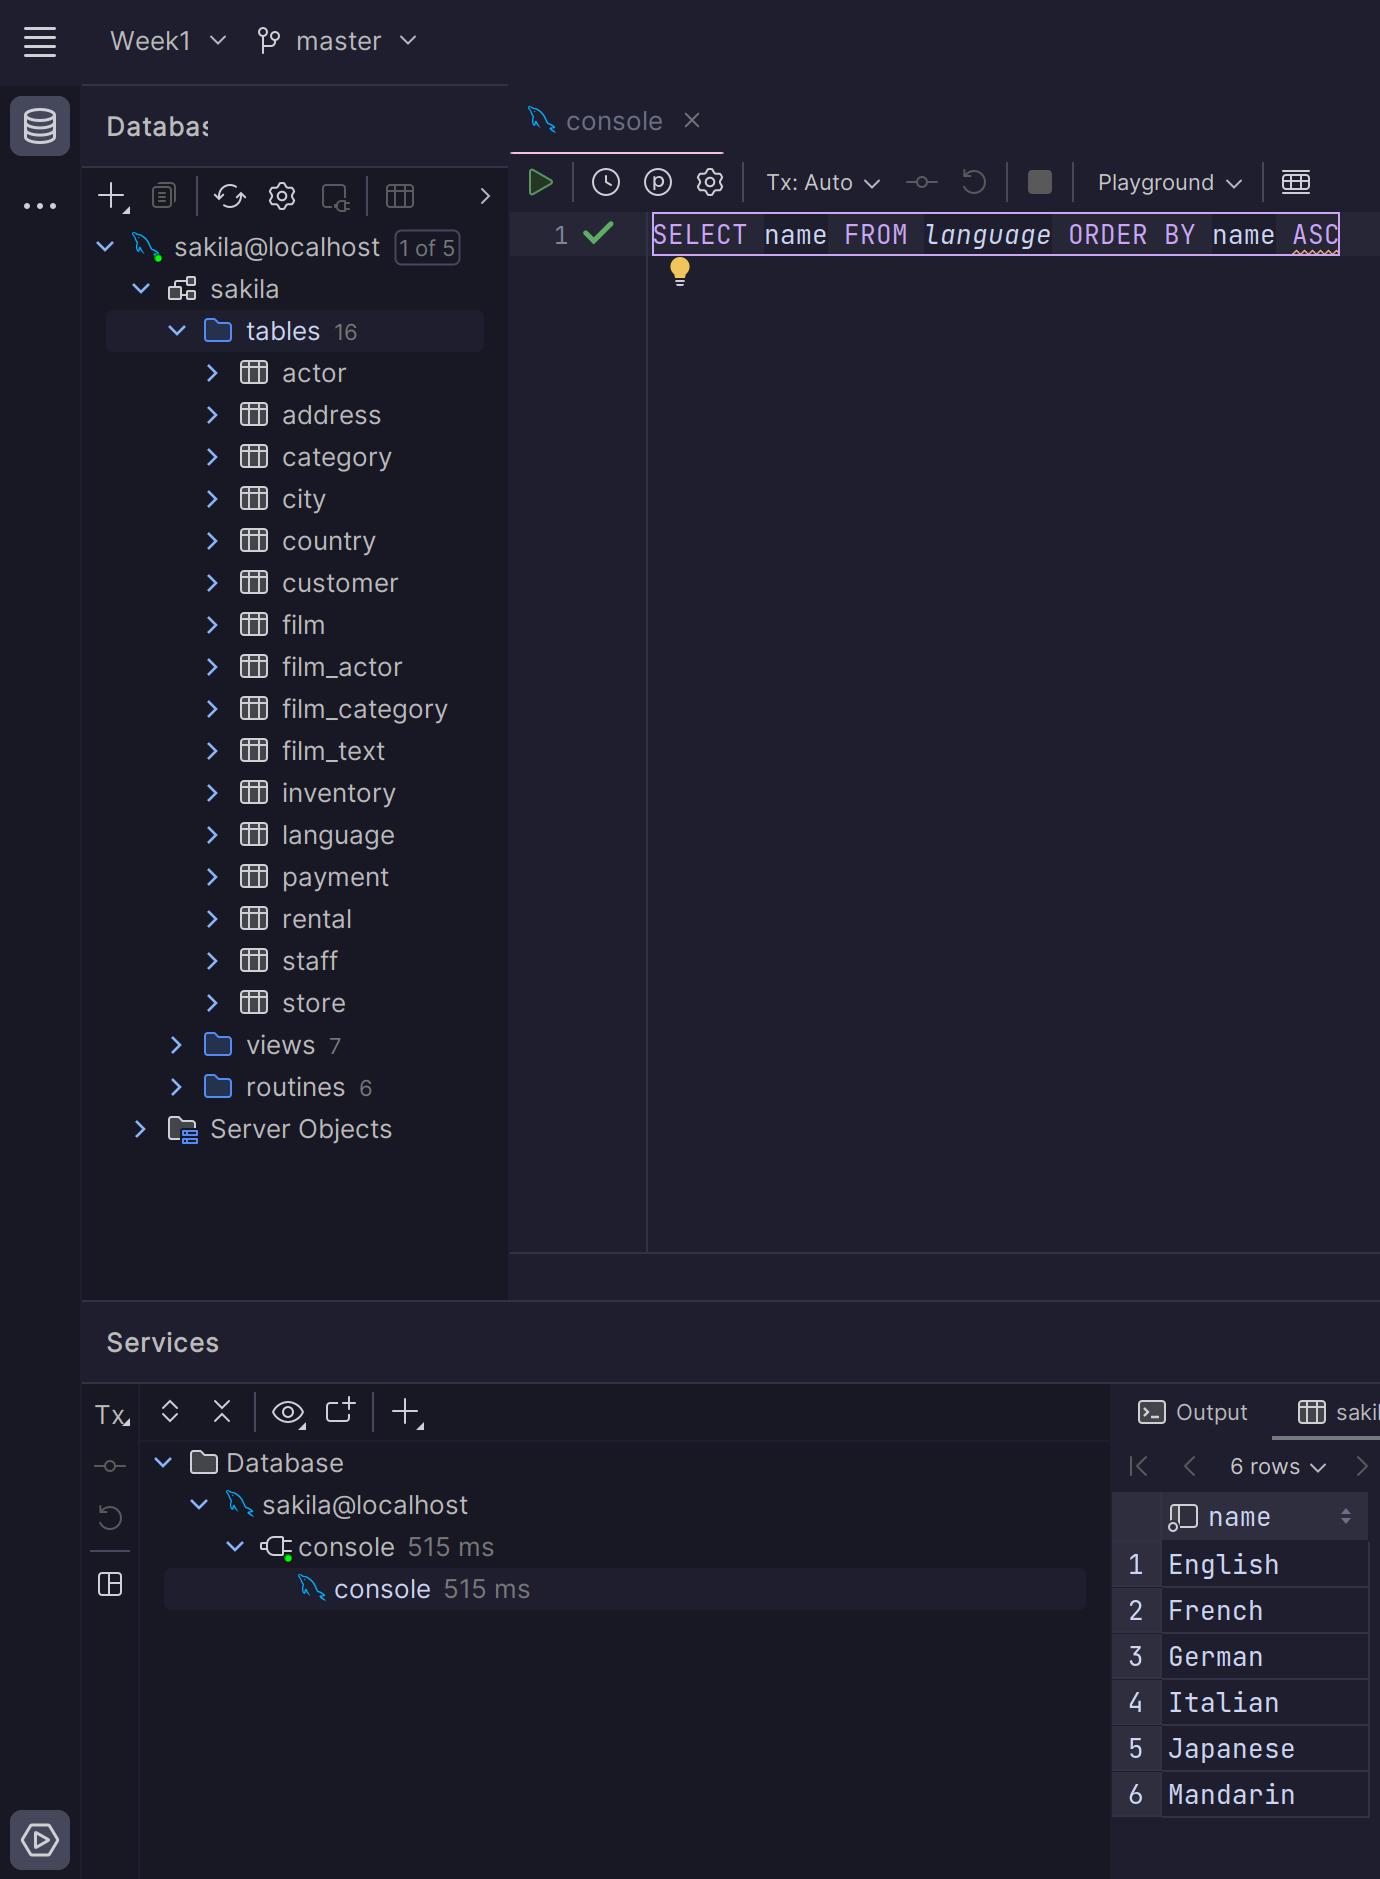
\includegraphics[width=\textwidth,height=\textheight,keepaspectratio]{question1}
	\question
	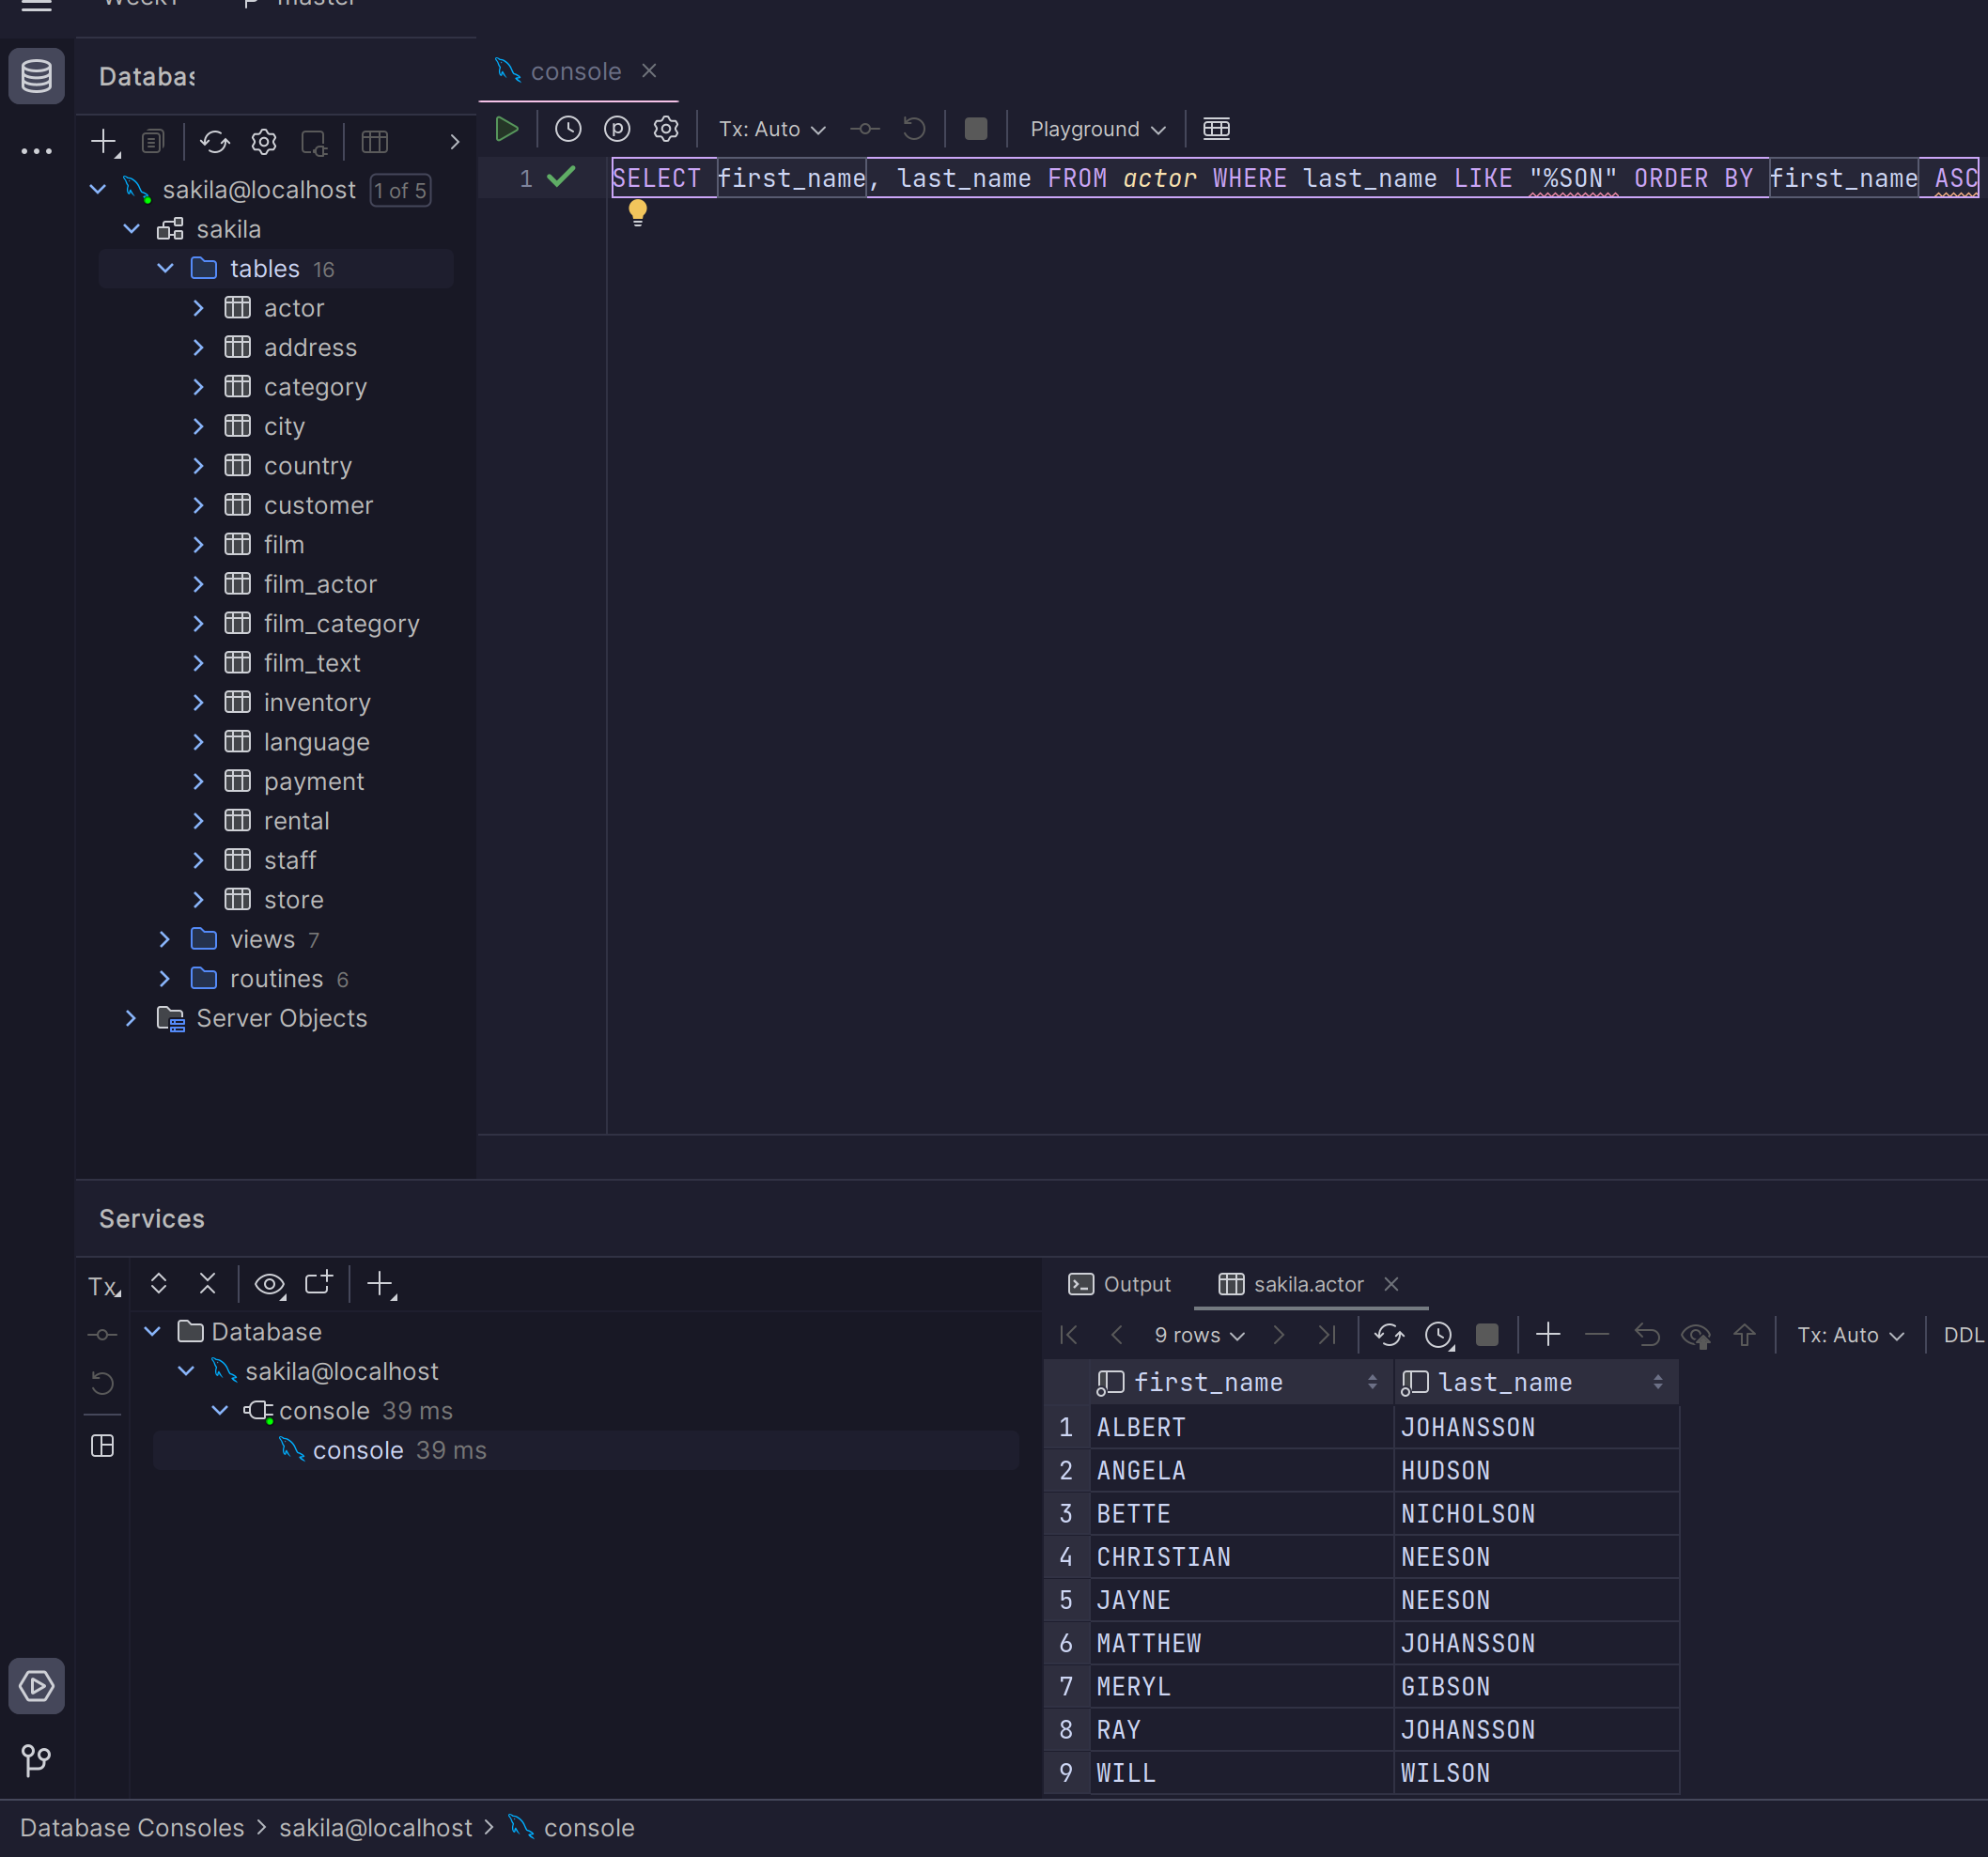
\includegraphics[width=\textwidth,height=\textheight,keepaspectratio]{question2}
	\question
	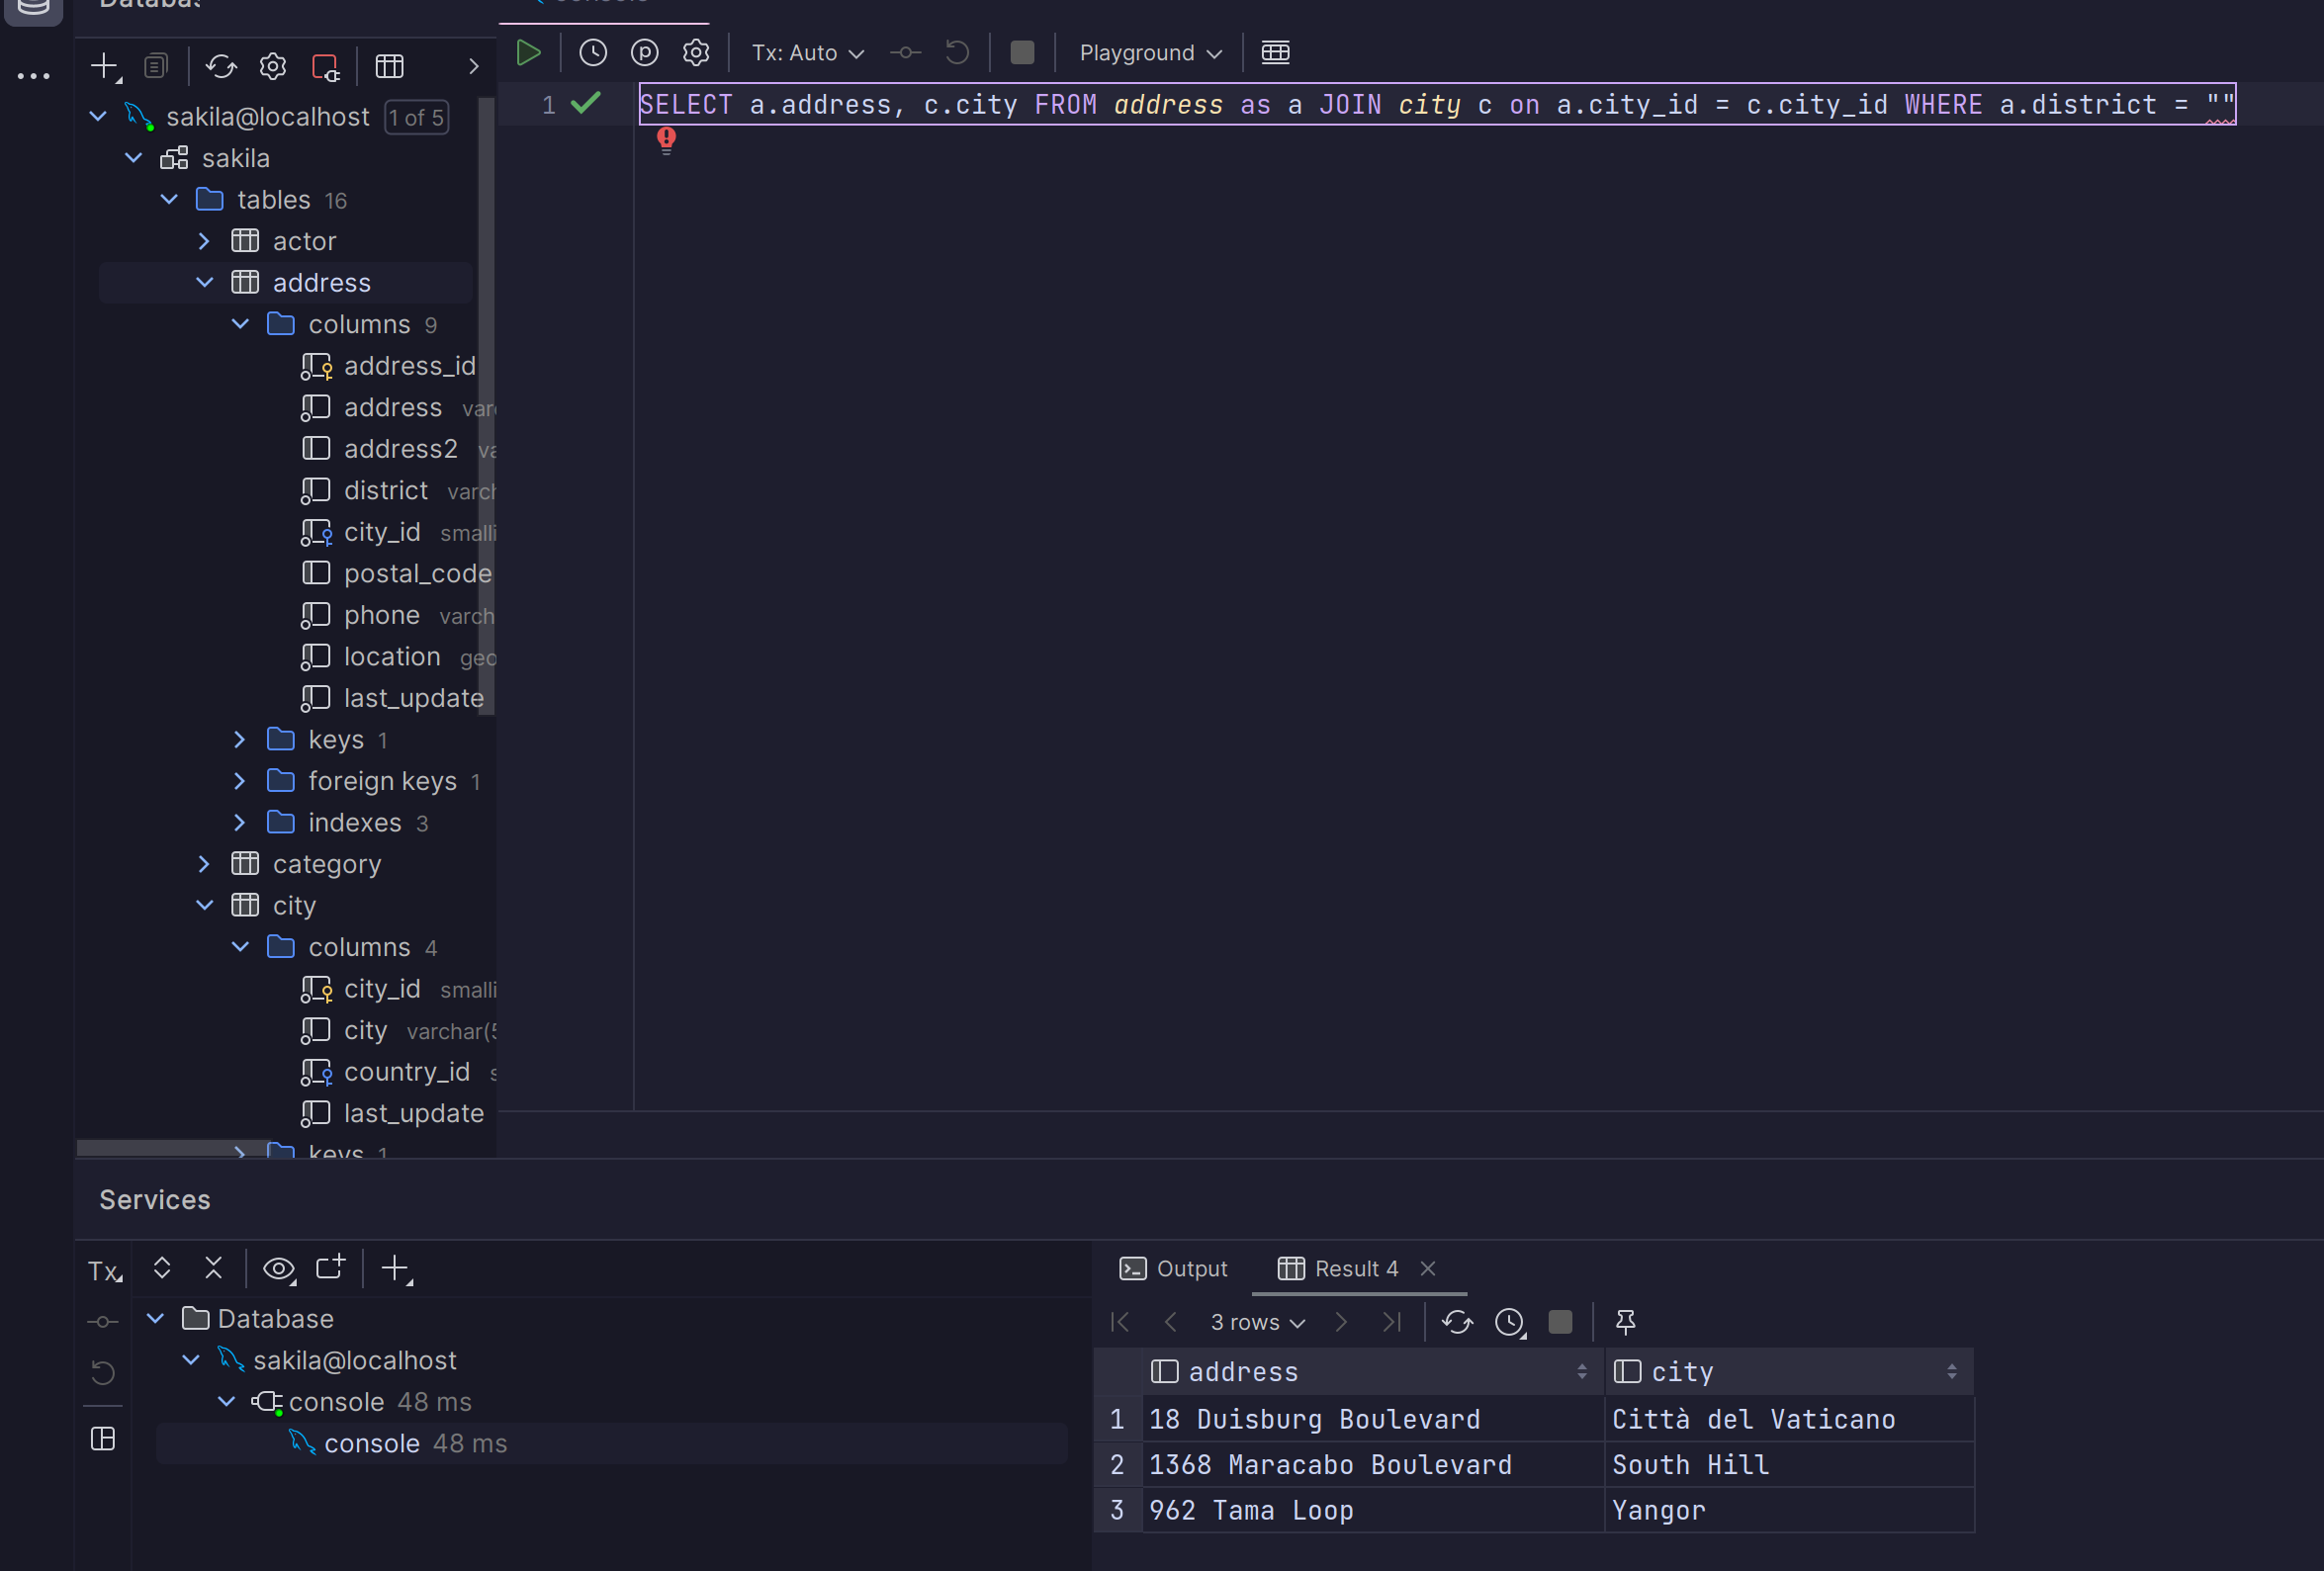
\includegraphics[width=\textwidth,height=\textheight,keepaspectratio]{question3}
	\question
	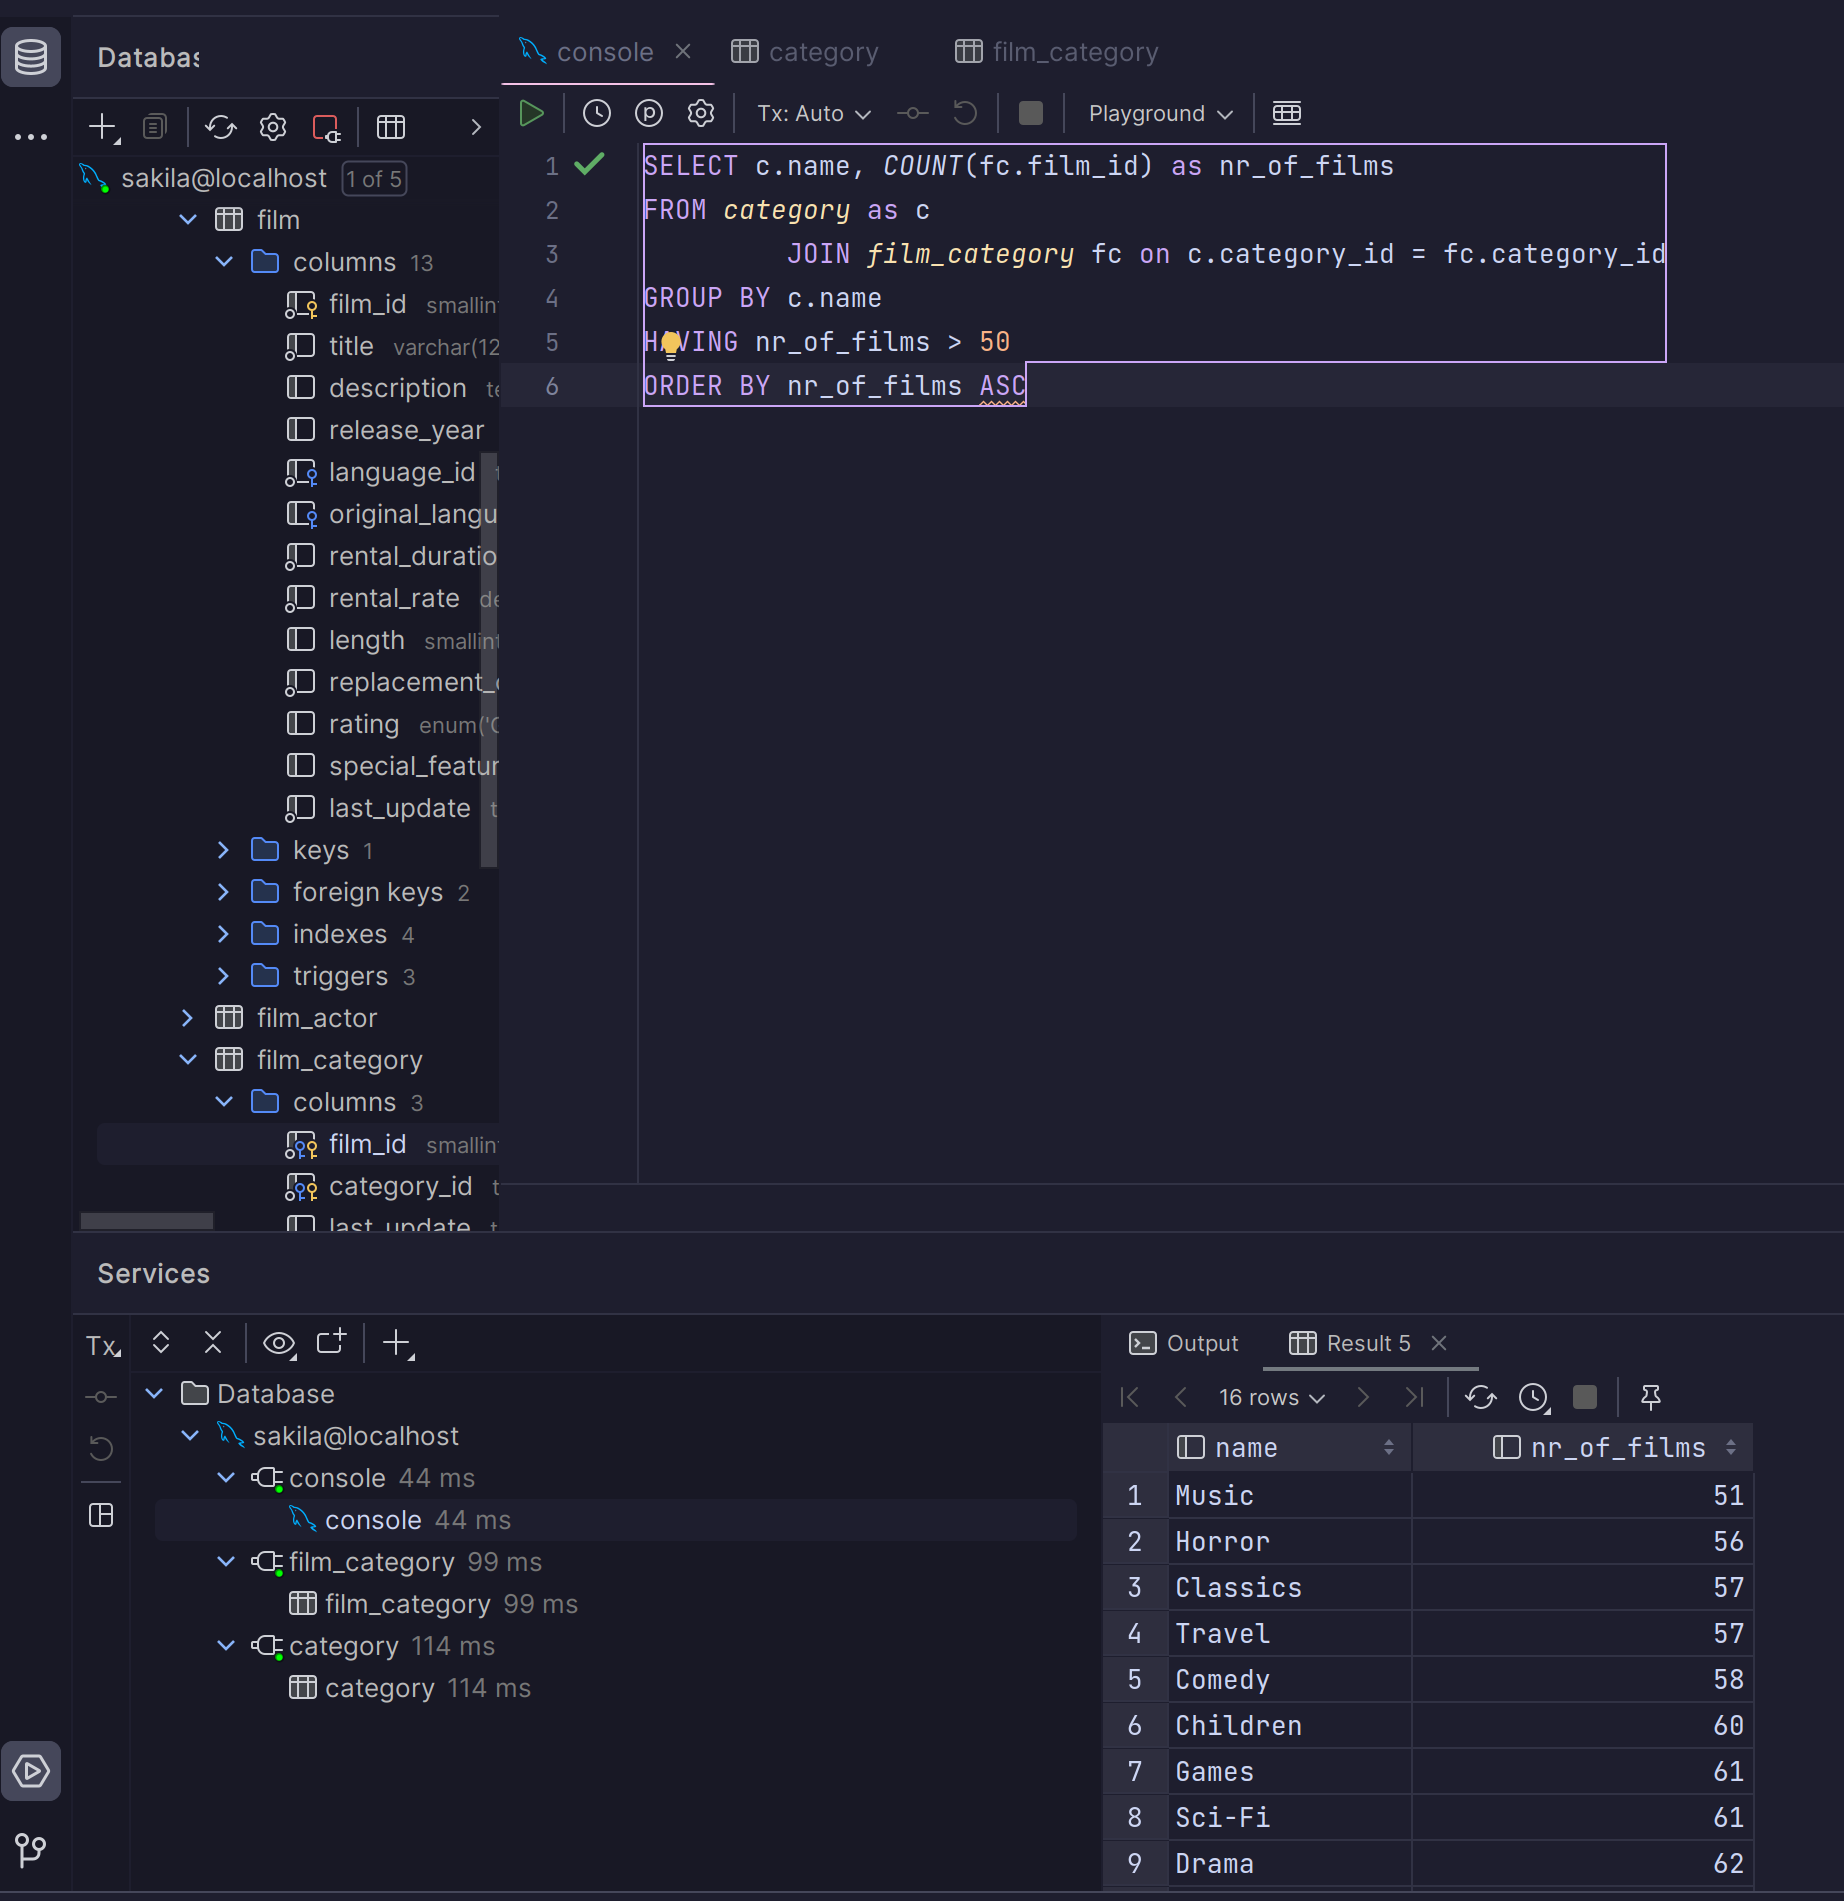
\includegraphics[width=\textwidth,height=\textheight,keepaspectratio]{question4}
	\question
	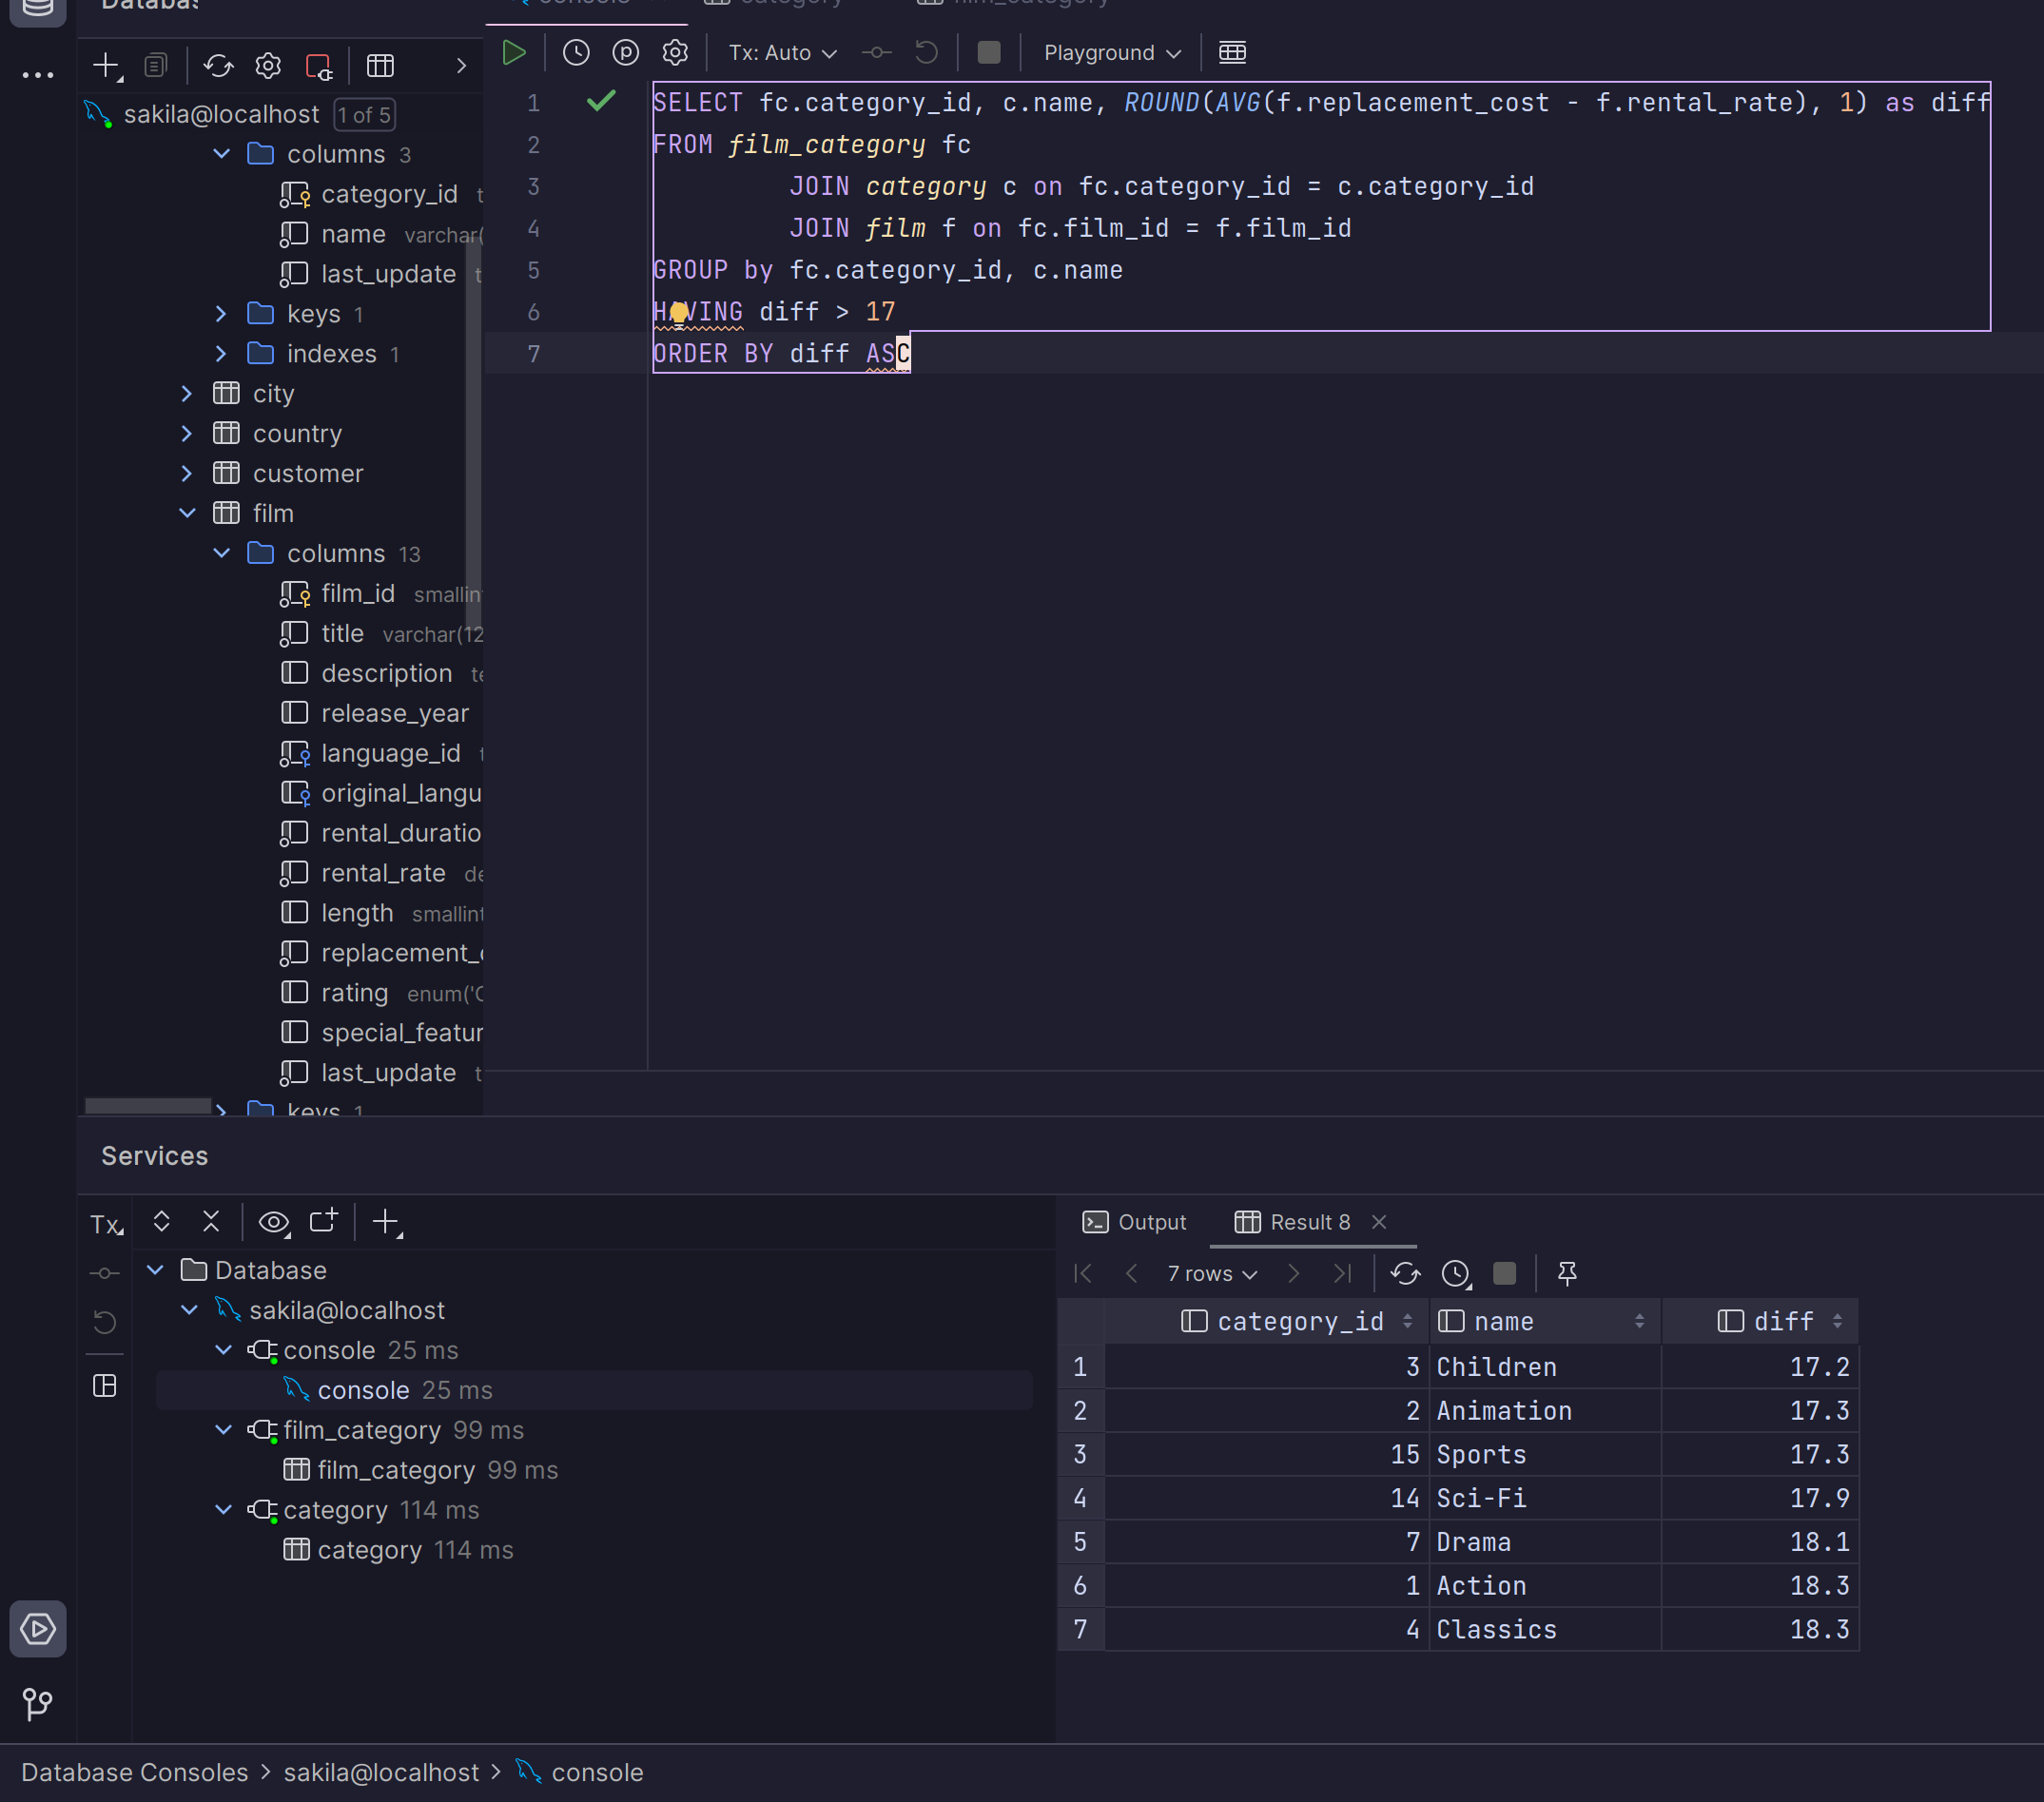
\includegraphics[width=\textwidth,height=\textheight,keepaspectratio]{question5}
	\question
	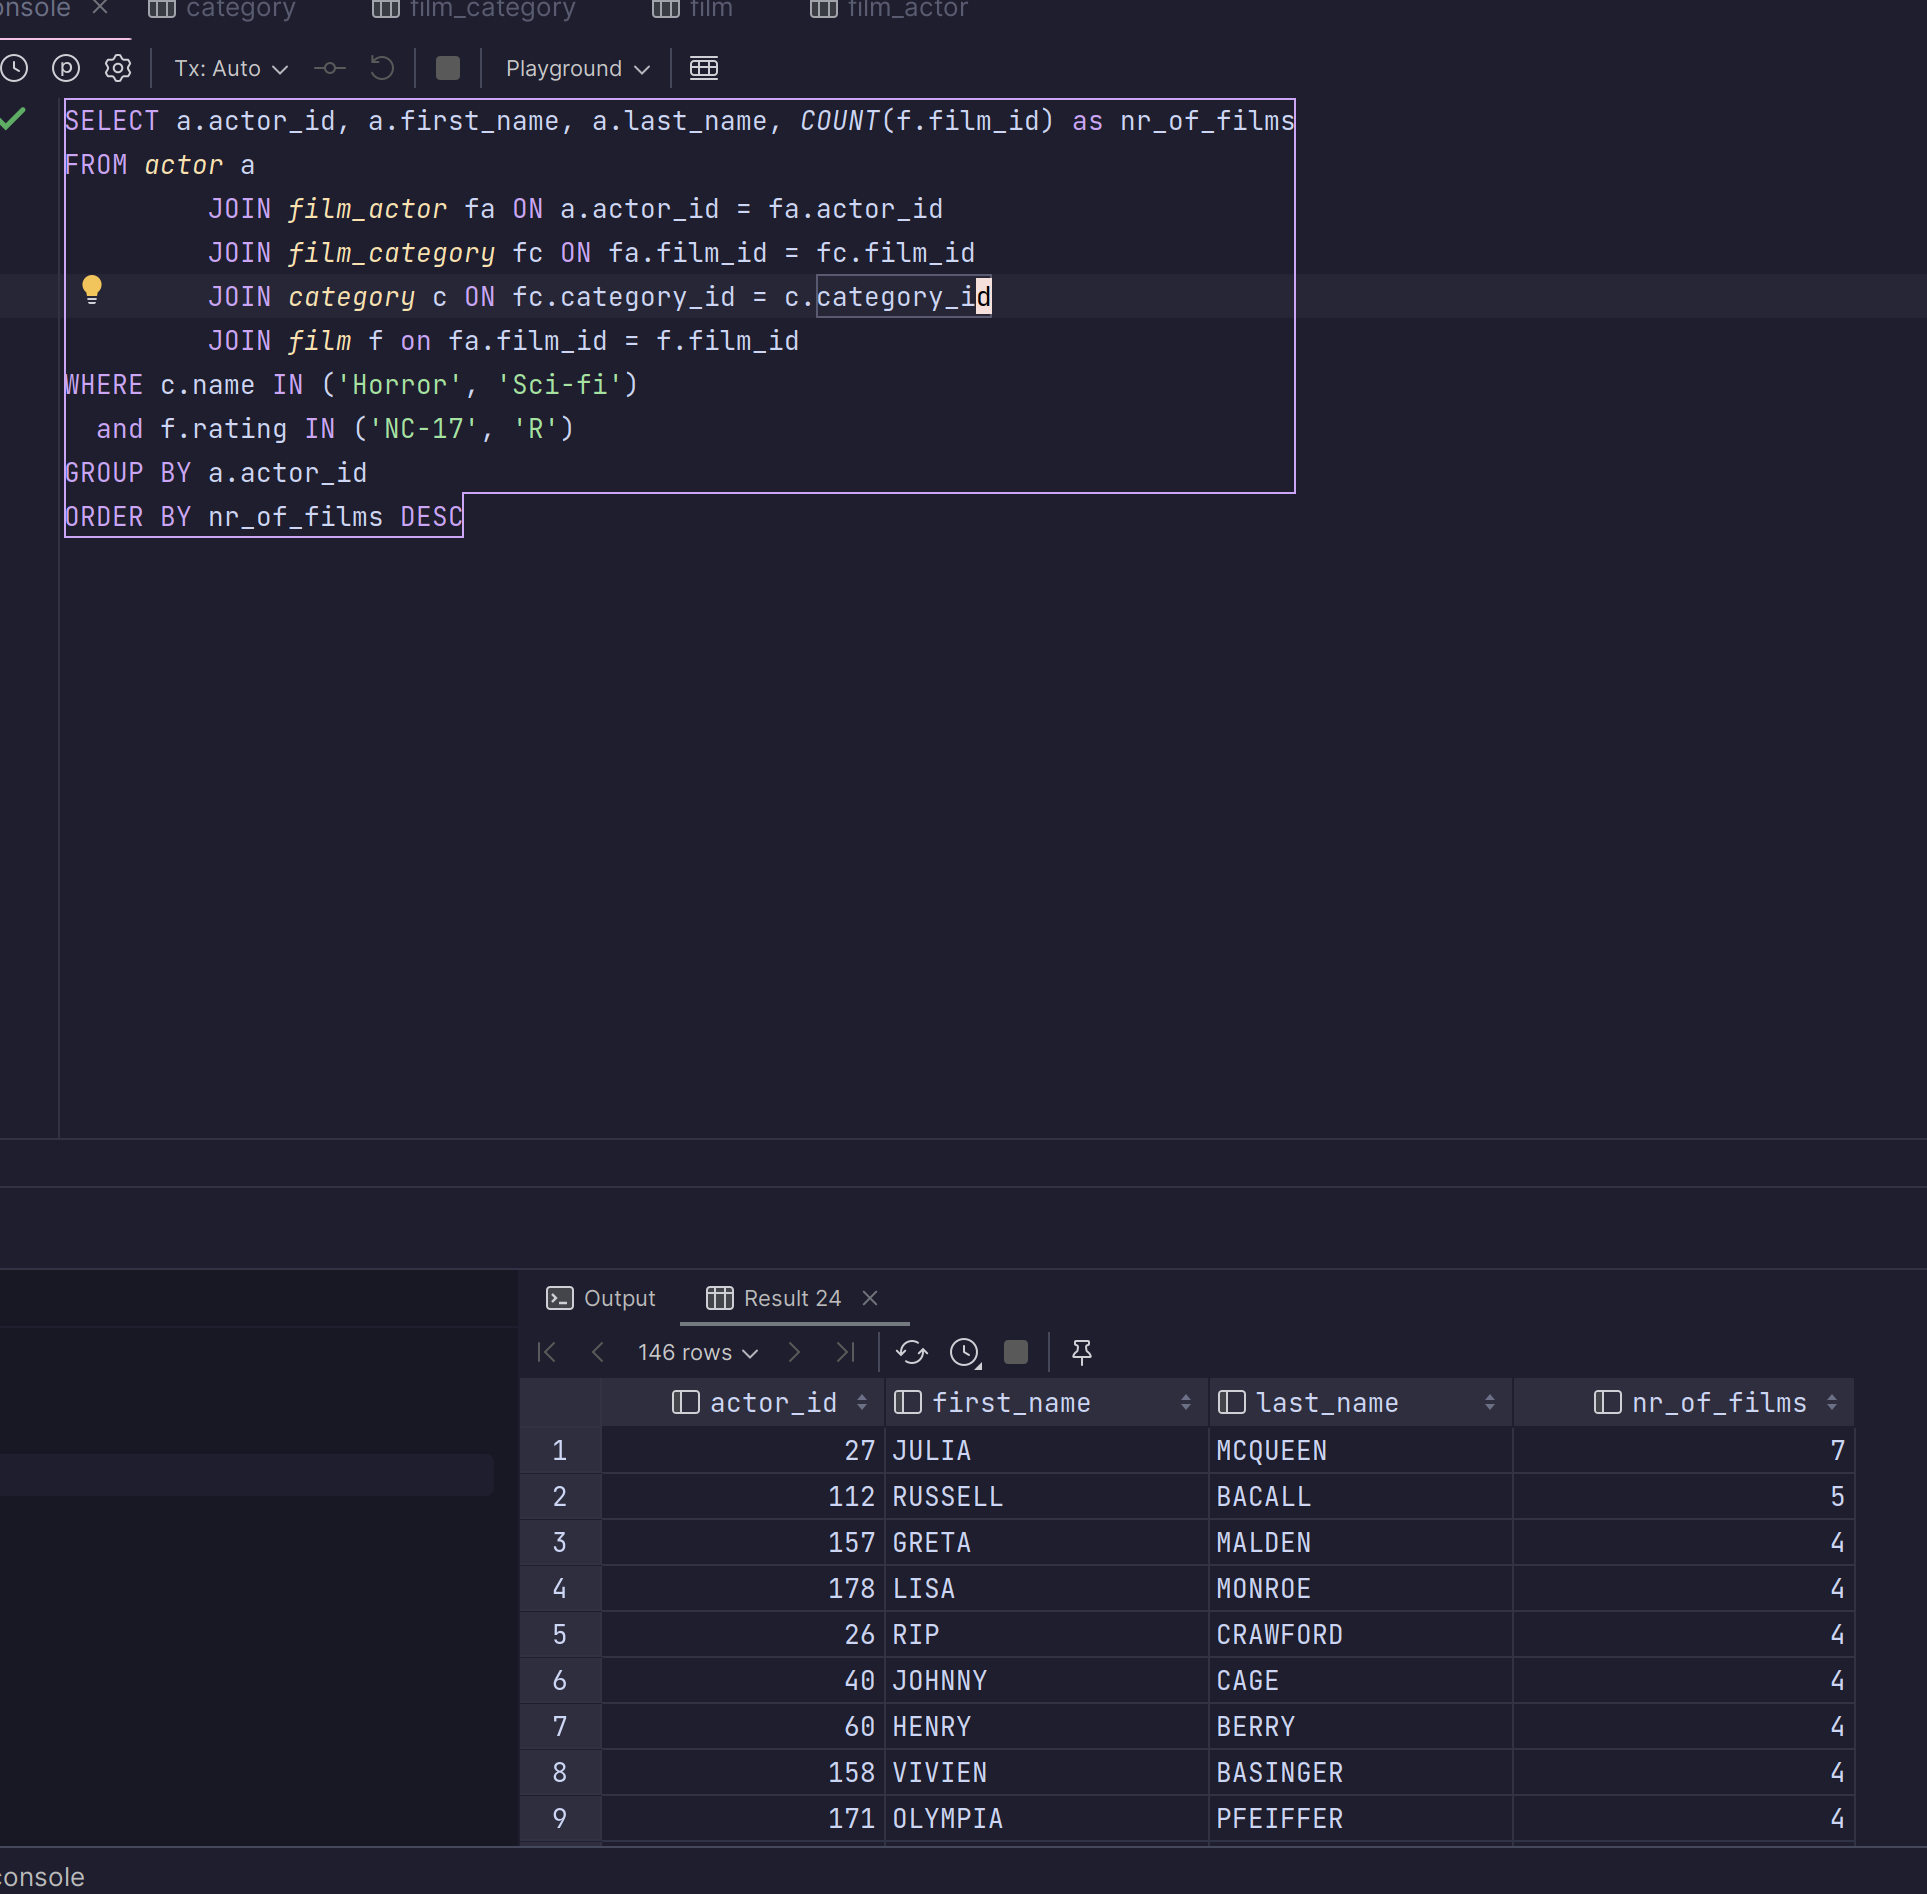
\includegraphics[width=\textwidth,height=\textheight,keepaspectratio]{question6}
	\question
	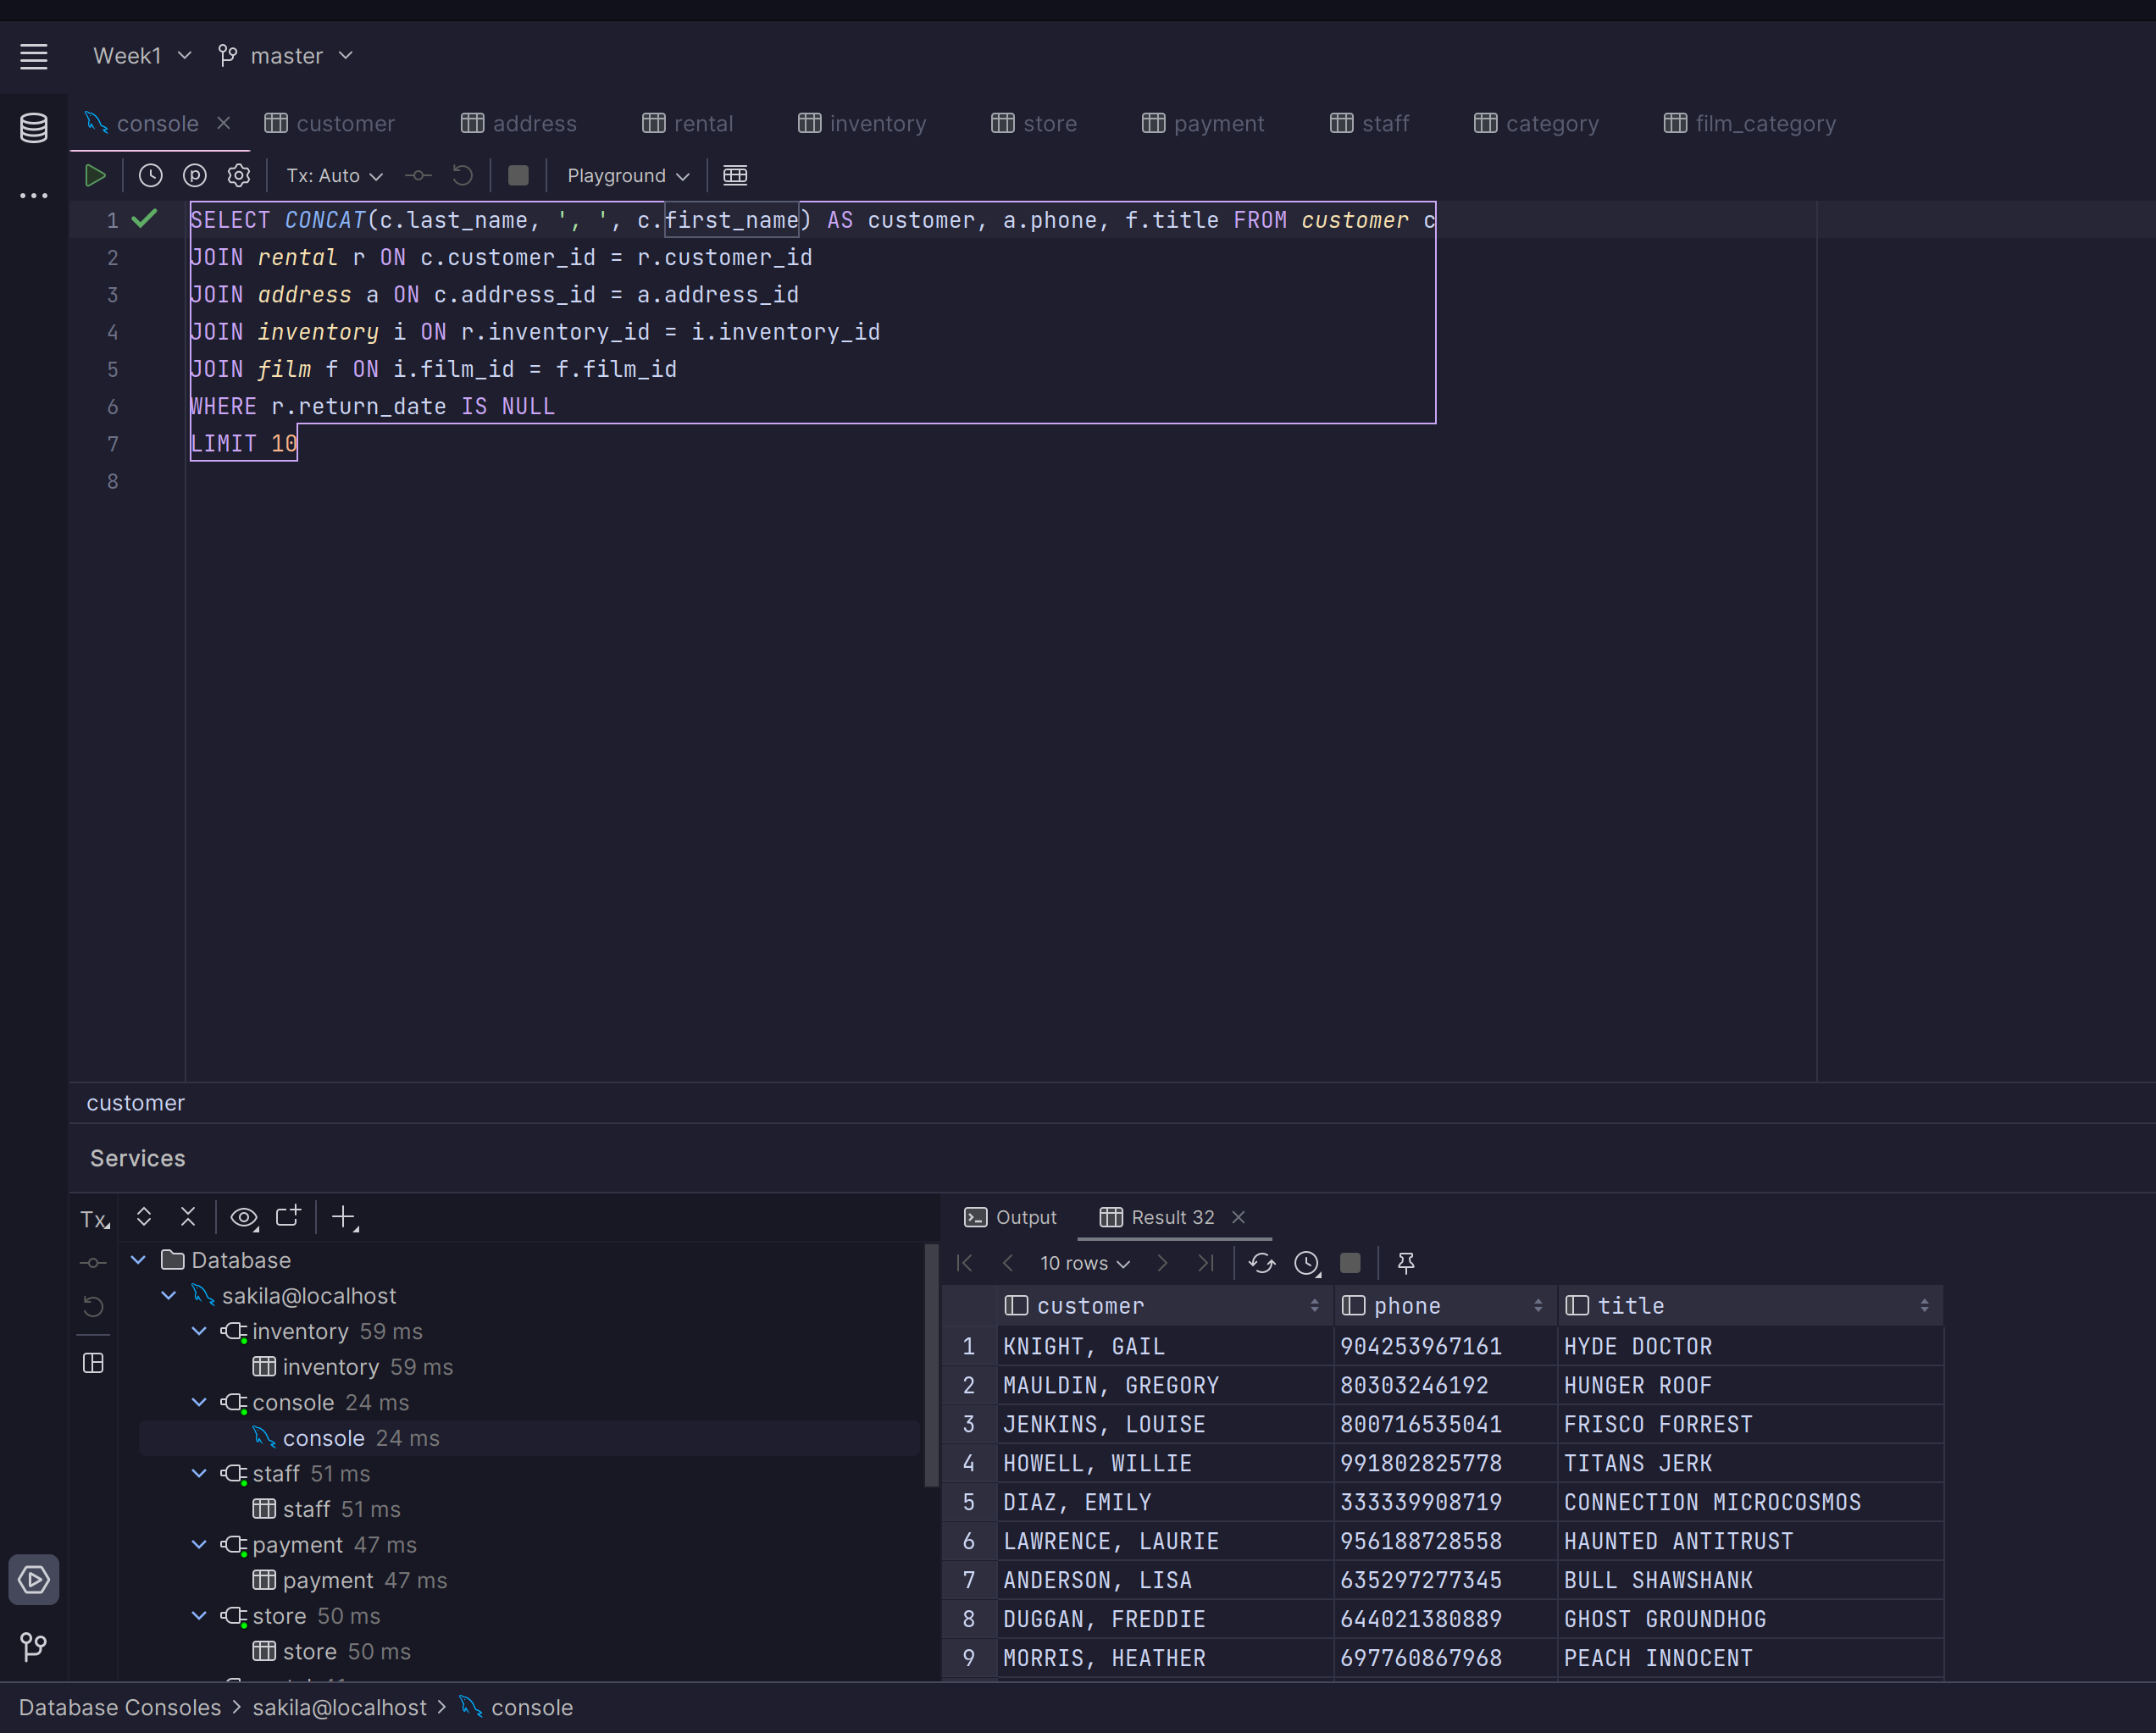
\includegraphics[width=\textwidth,height=\textheight,keepaspectratio]{question7}
	\question
	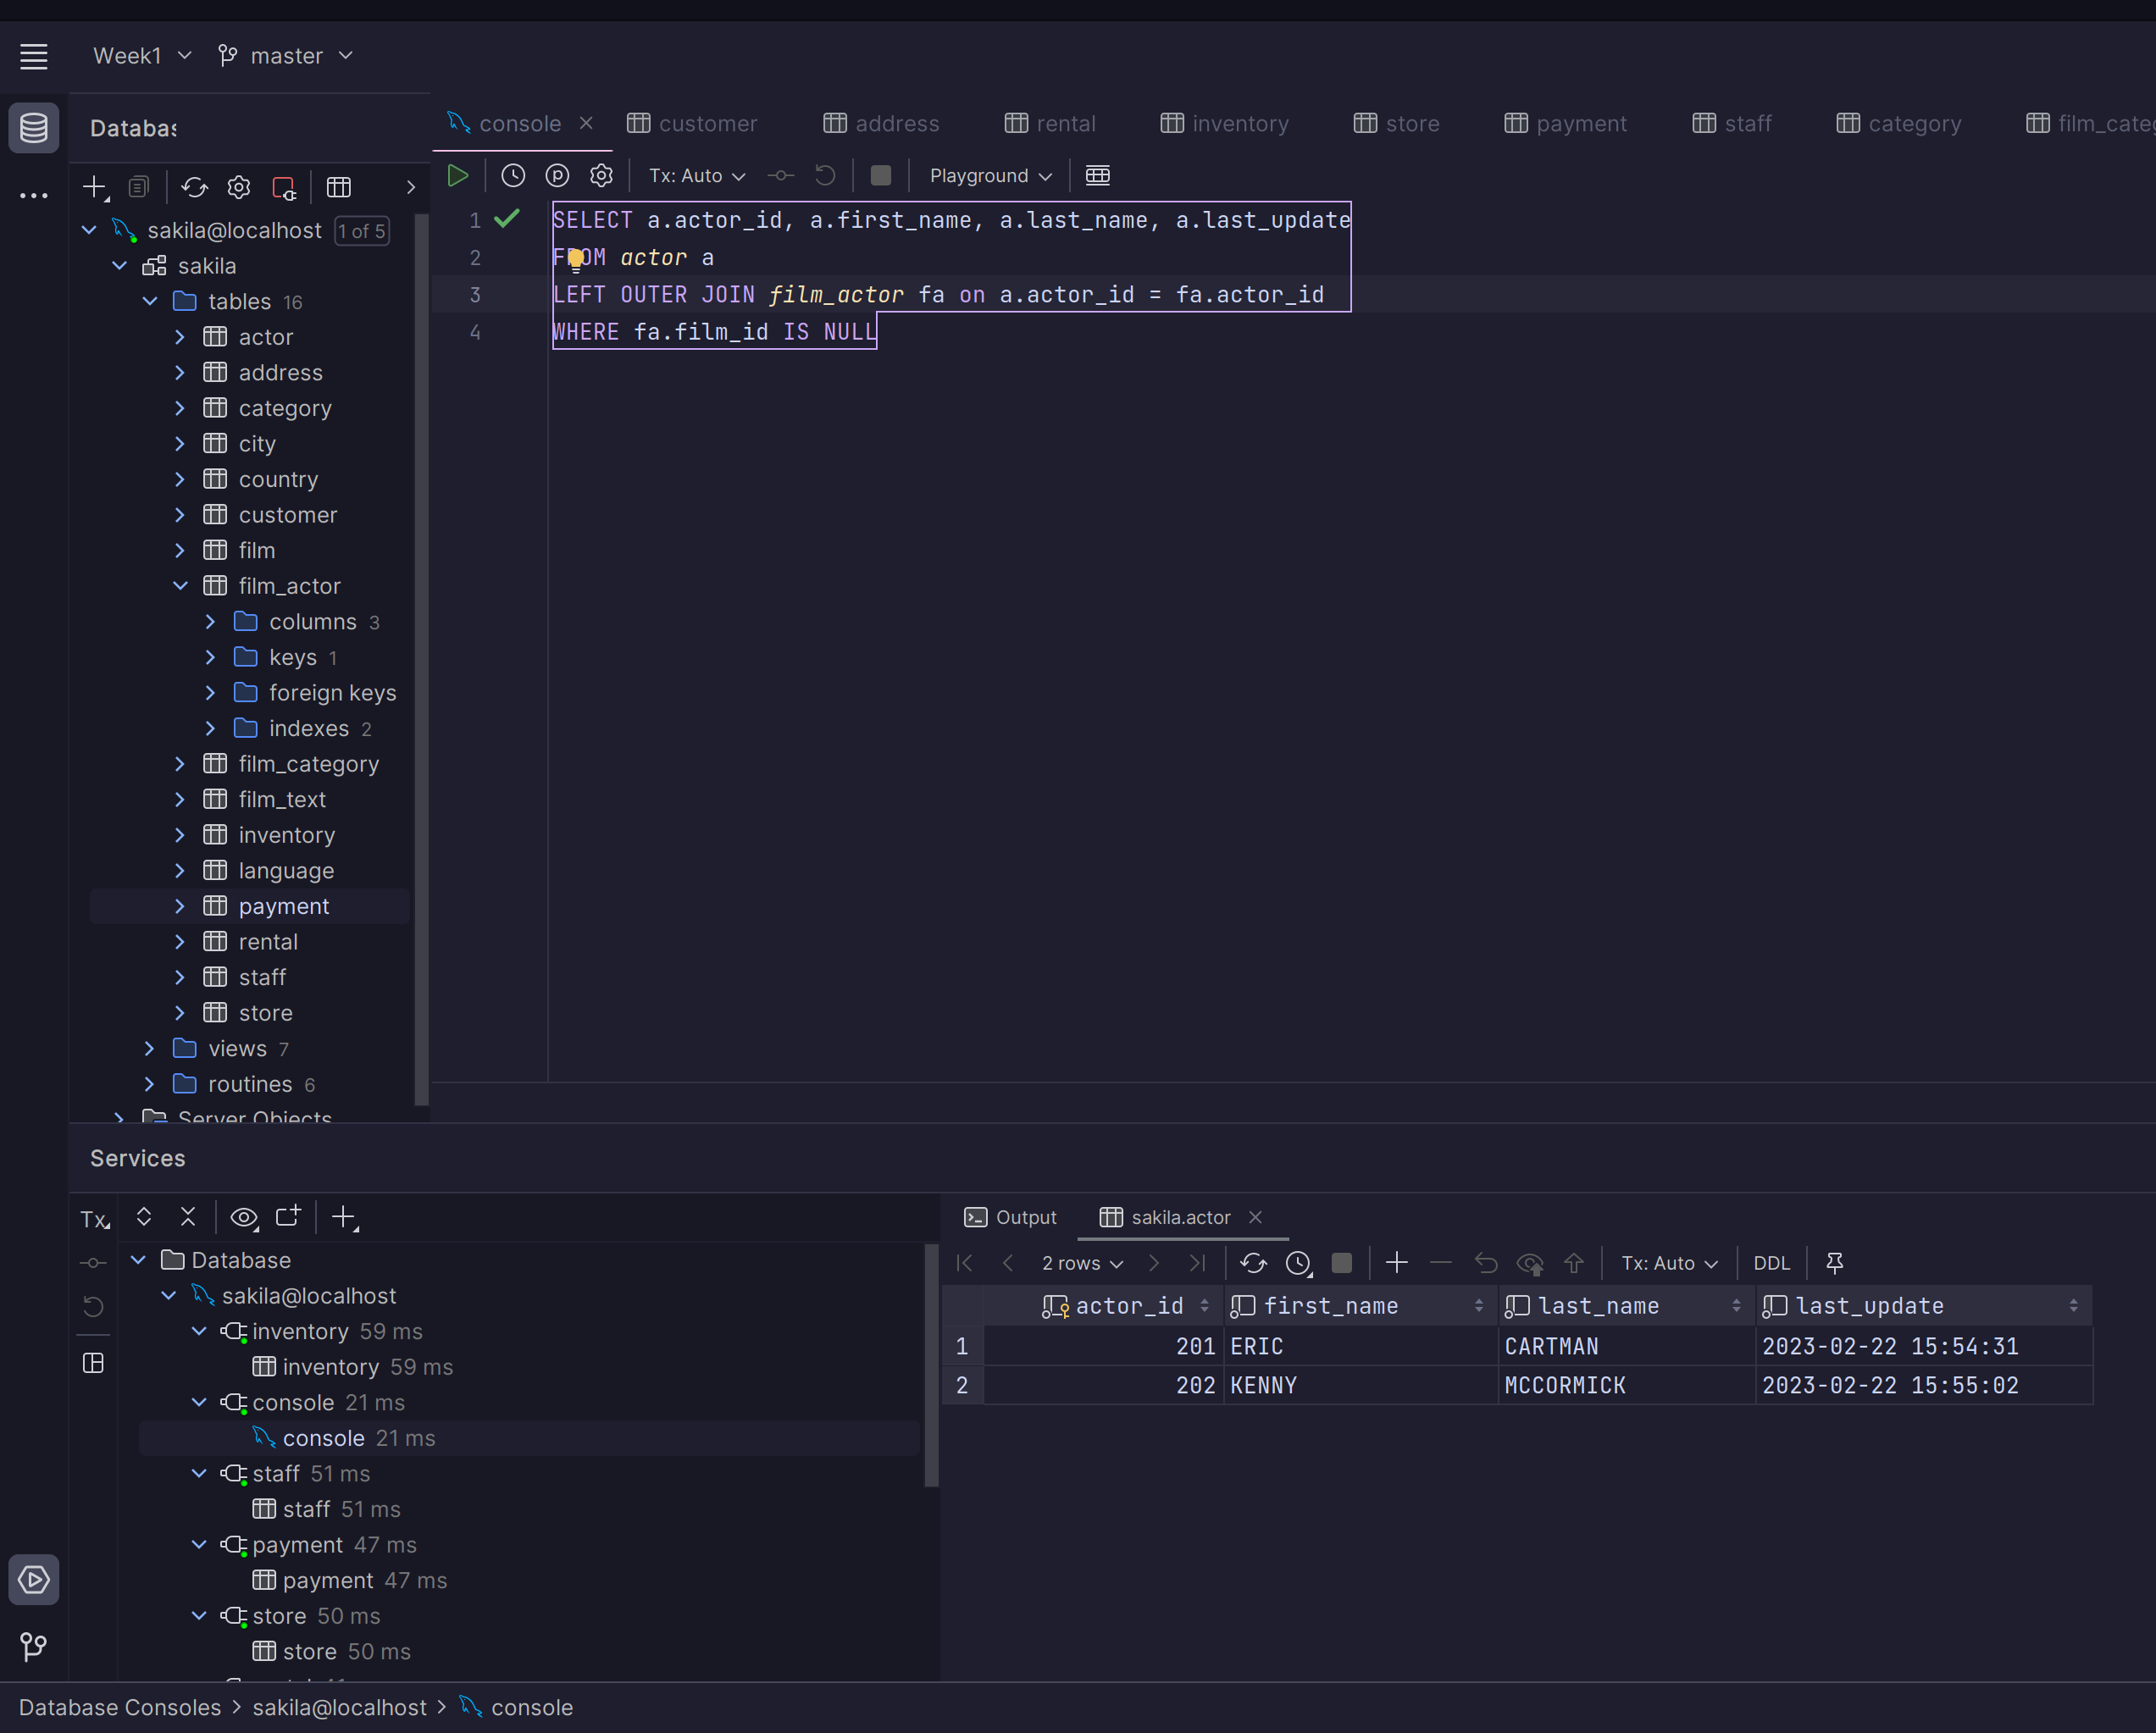
\includegraphics[width=\textwidth,height=\textheight,keepaspectratio]{question8}
	\begin{figure}
		\question
		\caption{Kan prima zonder}
		\centering
		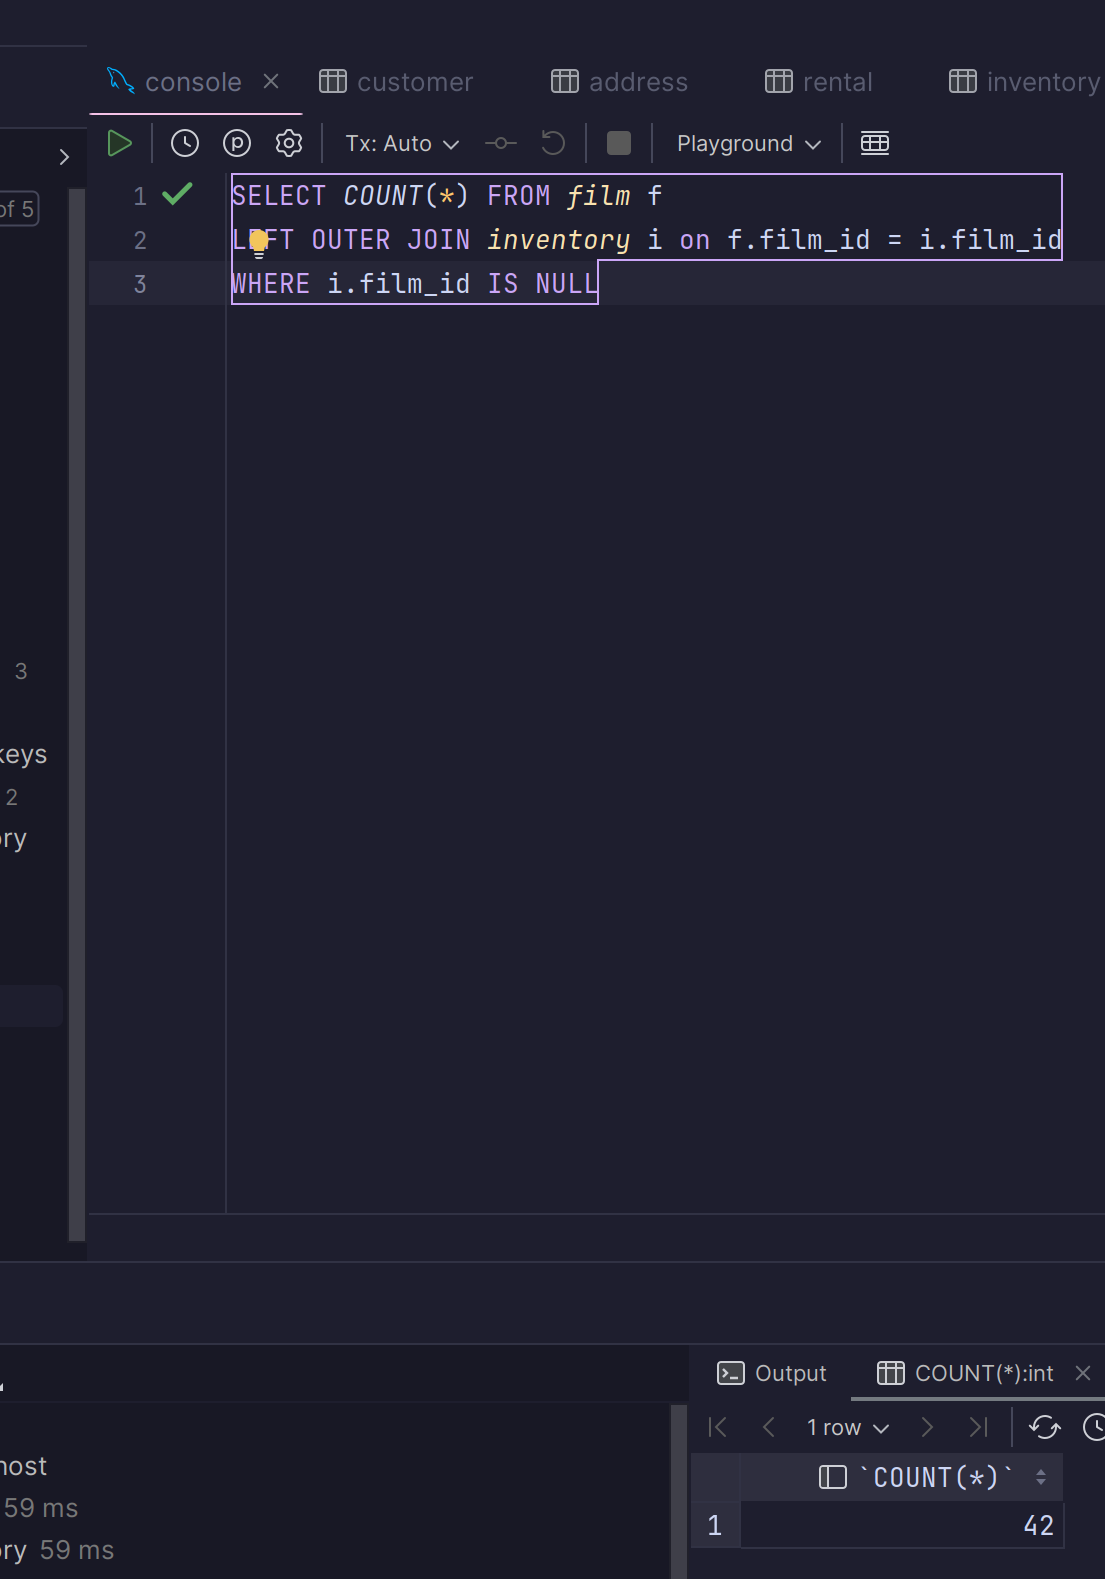
\includegraphics[width=\textwidth,height=\textheight,keepaspectratio]{question9}
	\end{figure}
	\question
	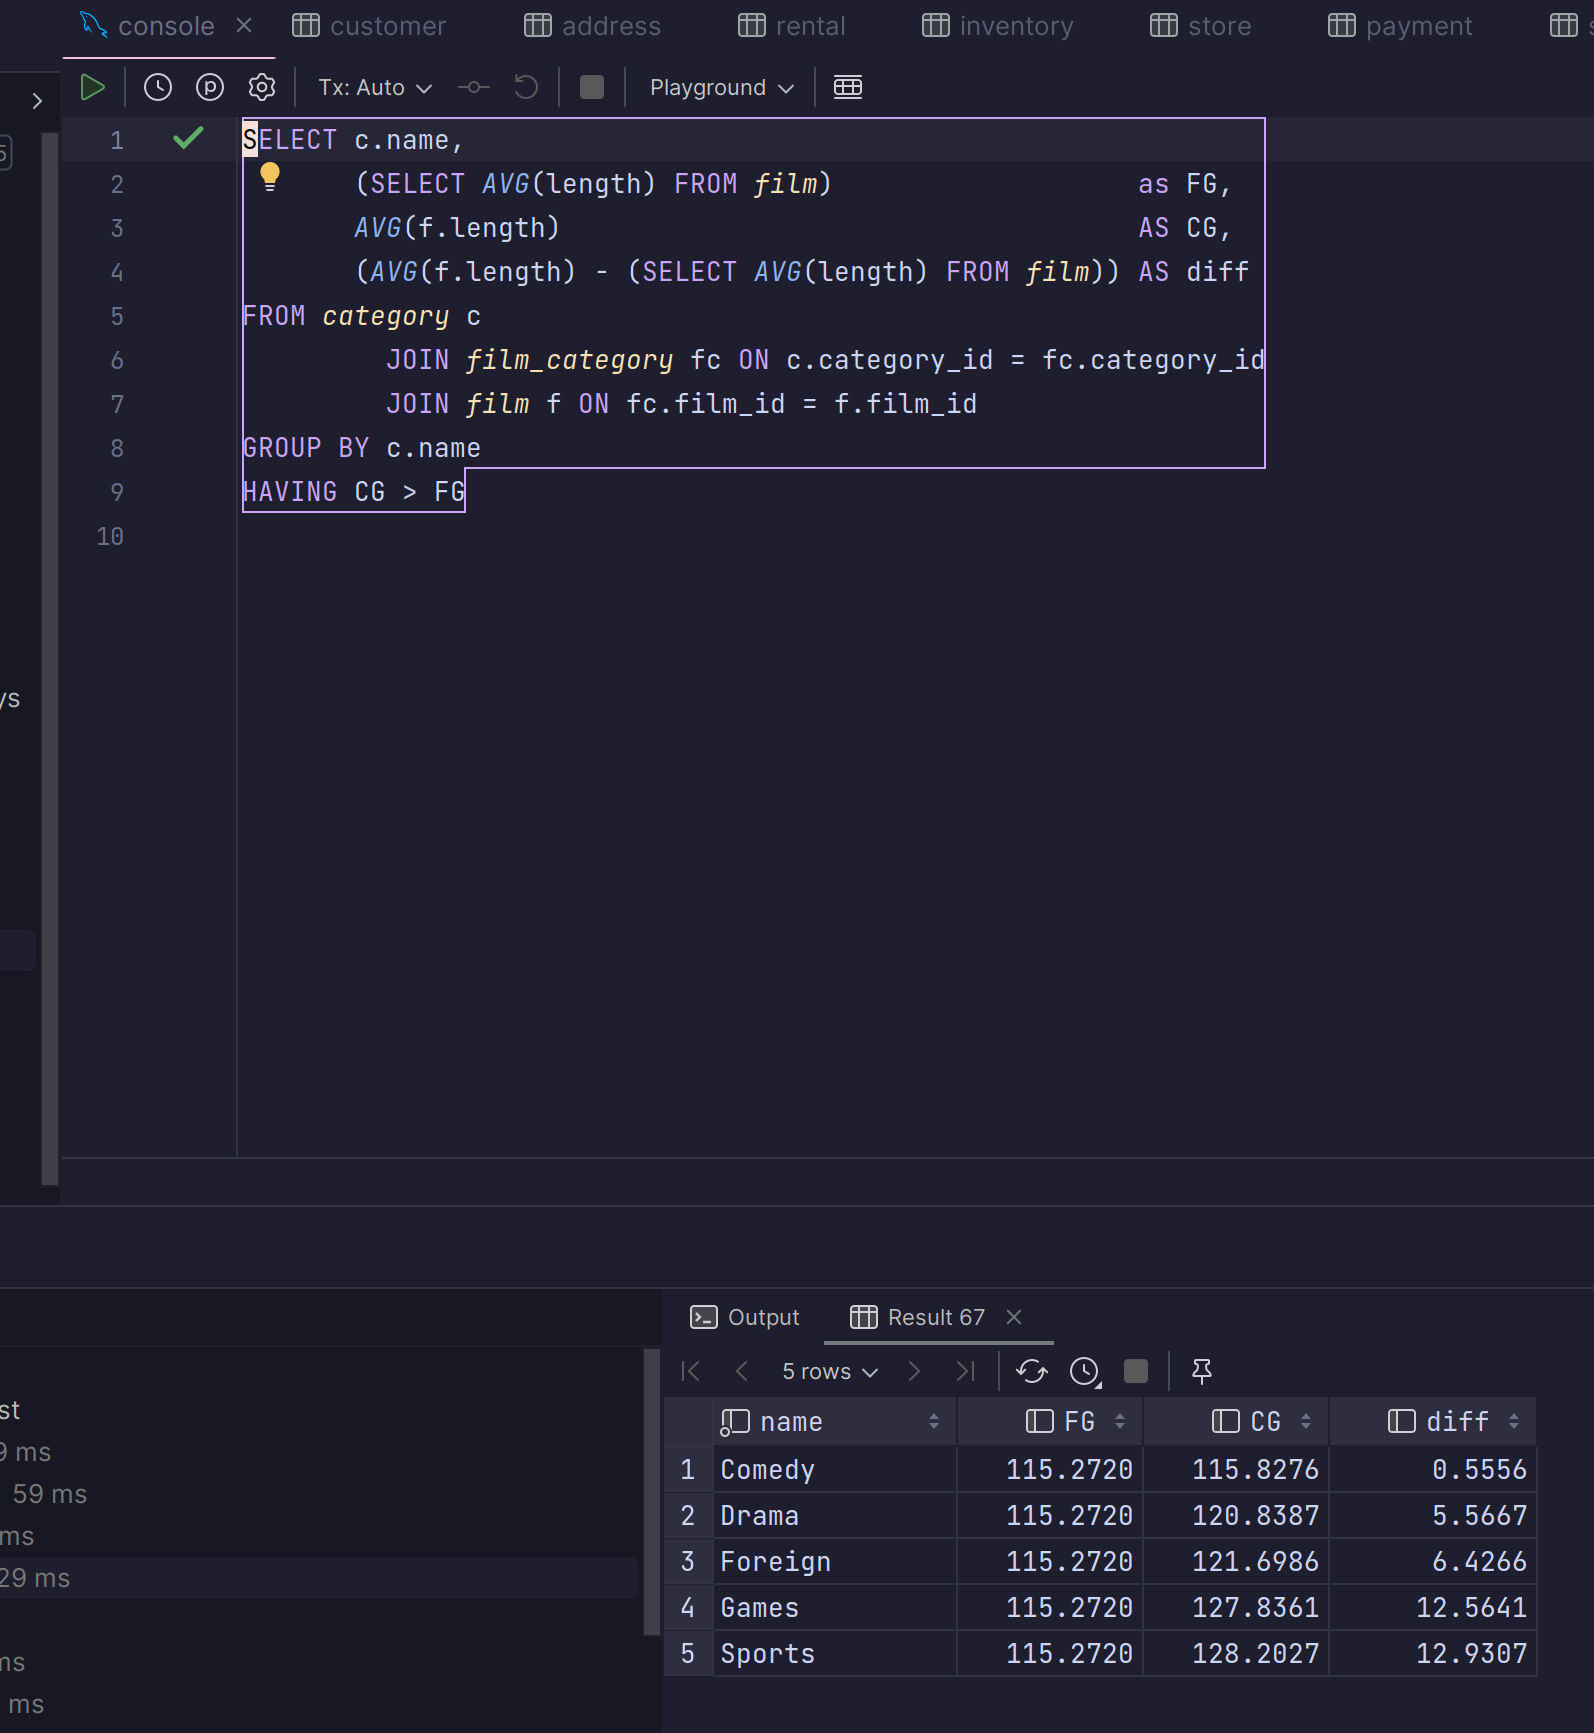
\includegraphics[width=\textwidth,height=\textheight,keepaspectratio]{question10}
\end{questions}
\end{document}
